\documentclass{article}
\usepackage{graphicx} 
\usepackage{amsmath}
\usepackage{amssymb}% Required for inserting images
\usepackage{amsfonts}
\usepackage[most]{tcolorbox}
\usepackage{amsthm}
\usepackage{cancel}
\newcommand{\prodscal}[2]{\vec{#1} \cdot \vec{#2}}
\usepackage[utf8]{inputenc}
\usepackage[T1]{fontenc}
\usepackage[italian]{babel}
\usepackage{geometry}
\geometry{a4paper ,  top = 2.5 cm , bottom = 2.5 cm, left = 2.5 cm , right = 2.5 cm}
\usepackage{changepage}
\usepackage{upgreek}
\usepackage{mathrsfs}
\usepackage{eufrak}
\usepackage{siunitx}
\usepackage{xcolor}
\usepackage{float}
\usepackage{textcomp}
\usepackage{comment}
\usepackage{titling}
\usepackage{parskip}
\usepackage{titlesec}
\usepackage{multicol}
\usepackage{subfigure}
\usepackage{wrapfig}
\usepackage{caption}
\usepackage{subcaption}
\usepackage{listings}
\usepackage{color}
\usepackage{numprint}
\npthousandsep{\,}
\usepackage{enumerate}
\usepackage{hyperref}
\hypersetup{
	colorlinks=true,
	linkcolor=blue,
	filecolor=magenta,      
	urlcolor=blue,
	pdftitle={},
	pdfpagemode=FullScreen,
}
\urlstyle{same}
\lstset{language=python,
	backgroundcolor=\color{white},
	basicstyle=\footnotesize\ttfamily,
	keywordstyle=\color{red},
	stringstyle=\color{codepurple},
	numberstyle=\tiny\color{codegray},
	breaklines=true,
	numbers=none,
	numberstyle=\scriptsize\sffamily\color{black},
	stepnumber=5,
	numbersep=10pt,
	captionpos=b,
	commentstyle=\footnotesize\ttfamily\color{blue}}
\lstset{frame=lines}
\lstset{label={lst:code_direct}}
\lstset{basicstyle=\footnotesize}
\setlength{\parindent}{0pt}
\addto\captionsitalian{\renewcommand*\figurename{\textsc{Fig.}}}
\addto\captionsitalian{\renewcommand*\tablename{\textsc{Tab.}}}

\usepackage{listings}

\lstset{
	language=C++,
	basicstyle=\ttfamily\small,
	keywordstyle=\color{blue},
	commentstyle=\color{gray},
	stringstyle=\color{orange},
	numbers=left,
	numberstyle=\tiny\color{gray},
	frame=single,
	breaklines=true
}

% Stile base per teoremi/definizioni
\tcbset{
	theobox/.style={
		enhanced,
		breakable,
		colback=gray!3!white,      % sfondo leggermente più scuro della pagina
		colframe=blue!60!black,     % bordo rosso scuro
		coltitle=blue!40!black,
		fonttitle=\bfseries,
		boxed title style={
			colback=blue!10!white,    % sfondo del titolo un po' più saturo
			boxrule=0.8pt
		},
		attach boxed title to top left={
			xshift=2mm,
			yshift=-2mm
		},
		top=3mm,
		bottom=3mm,
		left=3mm,
		right=3mm
		separator sign={}
	}
}

% Teorema
\newtcbtheorem[no counter]{teorema}{}%
{theobox}{th}

% Definizione (stesso stile, titolo diverso)
\newtcbtheorem[no counter]{definizione}{Definizione}%
{theobox, breakable=false}{defnb}

% Approfondimenti (verde)
\newtcolorbox{approfondimento}[2][]{%
	enhanced,
	breakable,
	colback=white!5!white,
	colframe=blue!50!black,
	coltitle=blue!40!black,
	fonttitle=\bfseries,
	title={#2},
	boxed title style={
		colback=white!10!white,
		boxrule=0.8pt
	},
	attach boxed title to top left={
		xshift=2mm,
		yshift=-2mm
	},
	top=3mm,
	bottom=3mm,
	left=3mm,
	right=3mm,
	#1
}


% Dimostrazioni (grigio chiaro, testo più piccolo)
\newtcolorbox{dimostrazione}[2][]{%
	enhanced,
	breakable,
	colback=gray!5!white,
	colframe=gray!50!black,
	coltitle=black,
	fonttitle=\bfseries,
	fontupper=\small,            % testo dentro la dimostrazione in \small
	title={#2},
	boxed title style={
		colback=gray!15!white,
		boxrule=0.6pt
	},
	attach boxed title to top left={
		xshift=2mm,
		yshift=-2mm
	},
	top=2mm,
	bottom=2mm,
	left=3mm,
	right=3mm,
	#1
}

\title{Metodi numerici per la fisica: \\ equazioni differenziali}
\author{Nicolò Mone}



\begin{document}
	
	\maketitle
	
	\tableofcontents
	
	\newpage
	\section{Introduzione all'analisi numerica nell'integrazione}
	Il problema dell'integrazione numerica può essere risolto, in linea di principio, con l'aiuto di equazioni differenziali ordinarie (\underline{ODEs}):
	\[ \int^x_a\, f(y)\, dy\ =\ g(x) \quad \quad \Rightarrow \quad \quad \frac{d\, g}{d\, x}\ =\ f(x)\ , \]
	con boundary $x_0=a$.
	
	Sebbene questa osservazione sia formalmente corretta, è preferibile sviluppare metodi diretti di integrazione numerica, analogamente a quanto si è fatto per le equazioni differenziali, dove la scelta del metodo appropriato non è affatto immediata.
	
	Un algoritmo generale di integrazione numerica ha la struttura
	
	\[
	\int_a^b f(x)\,dx = \sum_i w_i f(x_i),
	\]
	
	dove $w_i$ sono pesi e $x_i$ i nodi di valutazione. 
	
	In genere si pone $x_i = a + i h$ con passo $h$ uniforme e si scrive $f_i = f(x_i)$.
	
	\begin{multicols}{2}	
	Si distinguono due grandi classi di formule:
	
	\begin{itemize}
		\item \textbf{Formule chiuse}: utilizzano anche i valori agli estremi $a$ e $b$.
		\item \textbf{Formule aperte}: non utilizzano uno o entrambi gli estremi.
	\end{itemize}
	
	Il vantaggio principale delle formule aperte è che possono essere utilizzate quando la funzione non è definita agli estremi, pur essendo l'integrale ben definito.
	
	\begin{figure}[H]
		\centering
		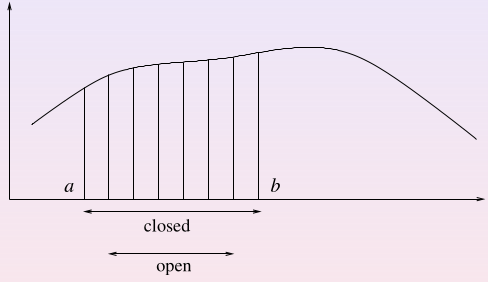
\includegraphics[width=\linewidth]{img/integration_1.png}
		\caption{differenza fra intervalli presi in considerazione da classi di formule chiuse e aperte}
	\end{figure}
	\end{multicols}
	
	
	
	\subsection{Formule di Newton–Cotes su intervallo singolo}
	
	Le formule di Newton-Cotes nascono dalla divisione in intervalli equispaziati e dalla successiva integrazione esatta di un polinomio che passa per quegli $n$ punti (interpolazione).
	
	La regola fondamentale dell'integrazione numerica, la formula di Newton-Cotes di grado più basso è la \underline{regola dei trapezi}, che usa una retta tesa fra due punti successivi per interpolare:
	
	\begin{equation}
		\label{trapezoidal-rule}
		\int_{x_1}^{x_2}\, f(x)\, dx\ =\
		\frac{1}{2}\, h \, [f_1 + f_2] + \mathcal{O}(h^3\, f^{''})\ ,\
	\end{equation}  
	
	questa è esatta per funzioni lineari, ad esempio $f(x)=x$. 
	
	Si ottiene interpolando $f(x)$ con il polinomio lineare che passa per i punti $(x_1,\, f_1)$ e $(x_2,\, f_2)$:
	
	\[ f(x)\ =\ f_1\, +\, (f_2\, -\, f_1)\, x\ \ , \]
	
	e in seguito integrando sull'intervallo normalizzato $0 \le x \le 1$.
	
	Formule di ordine superiore si ottengono interpolando con polinomi di grado più elevato. Ad esempio,
	
	\begin{equation}\label{Simpson's rule}
		\int_{x_1}^{x_3}\, f(x)\, dx\ =\ h\, \left[
		\frac{1}{3}\, f_1\, +\, \frac{4}{3}\, f_2\, +\, \frac{1}{3}\, f_3\right]\, +\,	\mathcal{O}(h^5\, f^{(4)})\ \ ,
	\end{equation} 
	
	che è la \underline{regola di Simpson}, esatta per polinomi fino al terzo grado.
	La regola di Simpson nasce dall'interpolazione con una parabola $P(x)=Ax^x + Bx+C$ su tre punti equispaziati $x_0$, $x_1$, $x_2$ con funzione da integrare $f_0=f(x_0)$, $f_1$, $f_2$. Facciamo un cambio di variabile $t=x-x_i$ così che i tre punti diventino $t=0,\, h,\, 2h$, riscrivendo la parabola come $P(t)=at^2+bt+c$. Si va ora ad imporre che $P(t=0)=c=f_0$, mentre nel secondo punto $P(t=h)=ah^2+b^h+c=f_1$ e nel terzo $P(t=2h)=4ah^2+2bh+c=f_2$. Invertendo questo sistema di equazioni si trova che $c=f_0$, $a=\frac{f_2-2f_1+f_0}{2h^2}$ mentre $b=\frac{f_1-f_0}{h}-ah$.
	A questo punto l'integrale $\int_{x_0}^{x_2} f(x) dx\approx \int_0^{2h} P(t) dt= \int_0^{2h} at^2+bt+f_0 dt$ è facilmente sostituibile con le dovute sostituzioni di $a$ e $b$ nelle forme appena trovate e con una semplice integrazione del polinomio si ottiene proprio Simpson: $\int_{x_0}^{x_2} f(x) dx\approx \frac{h}{3} [f_0 + 4\,f_1 + f_2]$.
	
	Analogamente, per cinque punti la formula di Newton-Cotes diventa:
	
	\[ \int_{x_1}^{x_5}\, f(x)\, dx\ =\ h\, \left[ \frac{14}{45}\, f_1\, +\, \frac{64}{45}\, f_2\, +\, \frac{24}{45}\, f_3\, +\, \frac{64}{45}\, f_4\, +\, \frac{14}{45}\, f_5\, \right]\, +\, \mathcal{O}(h^7\, f^{(6)})\ \ .\]
	
	\subsection{Alcune formule locali}
	
	È utile osservare anche relazioni locali su intervalli elementari:
	
	\[ \int_{x_0}^{x_1}\, f(x)\, dx\ =\ h[f_1]\, +\, \mathcal{O}(h^2\, f')\ \ ,\]
	
	
	\[ \int_{x_0}^{x_1}\, f(x)\, dx\ =\ h\, \left[ \frac{3}{2}f_1\, -\, \frac{1}{2}f_2 \right]\, +\, \mathcal{O}(h^3\, f'')\ \ .\]
	
	La prima è un semplice rettangolo, una Newton-Cotes aperta di ordine 0 con errore di ordine $h^2$, mentre la seconda formula è una Newton-Cotes aperta di ordine 1 e si ottiene interpolando linearmente $f(x)\ =\ f_1 + x\, (f_2 - f_1)$, e integrando nell'intervallo $-1 \le x \le 0$:
	
	\[ \int_{-1}^{0} f(x)\,dx\ =\ -(-f_1)\, -\, \frac{(-1)^2}{2}\, (f_2 - f_1) \ =\ \left[ \frac{3}{2}f_1 - \frac{1}{2}f_2\right]\ .\]
	
	Formule di ordine superiore si ottengono usando approssimazioni polinomiali di grado crescente.
	
	\subsection{Intervalli estesi}
	
	Passando a intervalli estesi, dalla regola dei trapezi in eq.(\ref{trapezoidal-rule}) segue una regola dei trapezi estesa:
	
	\begin{equation} \label{regola-dei-trapezi-estesa}
		\int_{x_1}^{x_n} f(x)\,dx\ =\ h\, \left[
		\frac{1}{2}f_1\, +\, f_2\, +\, f_3\, +\, \dots\, +\, \frac{1}{2}f_n
		\right]\, +\,
		\mathcal{O}\!\left(\frac{(x_n-x_1)^3}{N^2}\, f''\right)\ \ ,
	\end{equation} 
	
	dove $N$ è il numero di suddivisioni.
	
	Dalla regola di Simpson in eq.(\ref{Simpson's rule}), si ottiene invece:
	
	\begin{equation}\label{Simpson-esteso}
		\int_{x_1}^{x_n}\, f(x)\,dx\ =\ h\, \left[ \frac{1}{3}f_1\,+\,\frac{4}{3}f_2\,+\,\frac{2}{3}f_3\,+\,\frac{4}{3}f_4\,\dots\,+\,\frac{4}{3}f_{n-1}\,+\,\frac{1}{3}f_n\right]
		\,+\,\mathcal{O}\!\left(\frac{1}{N^4}\right)\ \ .
	\end{equation} 
	
	Di seguito un'implementazione in C della regola dei trapezi e di Simpson:
	\lstinputlisting{trapezi.c}
	
	Si può combinare una formula aperta locale (singolo intervallo) con una formula chiusa estesa di quelle appena scritte per ottenere una formula aperta su intervallo esteso. 
	
	Ad esempio, combinando
	
	\[
	\int_{x_0}^{x_1} f(x)\,dx
	=
	h f_1 + \mathcal{O}(h^2 f')
	\]
	
	con la regola dei trapezi estesa su $[x_1,x_n]$ vista in eq.\ref{regola-dei-trapezi-estesa}, si ottiene:
	
	\[ \int_{x_0}^{x_n}\, f(x)\, dx\ =\ h\, \left[ \frac{3}{2}f_1\, +\, f_2\, +\, f_3\, +\, \dots\, +\, \frac{3}{2}f_{n-1}\right]\,+\, \mathcal{O}\!\left(\frac{1}{N^2}\right)\ \ .\]
	
	Analogamente, combinando la formula aperta di ordine superiore
	
	\[ \int_{x_0}^{x_1} f(x)\,dx \ =\ h\,\left[ \frac{23}{12}f_1\,-\,\frac{16}{12}f_2\,+\,\frac{5}{12}f_3\right]\, +\, \mathcal{O}(h^4 f^{(3)})\ \ , \]
	
	con la regola di Simpson estesa eq.(\ref{Simpson-esteso}), si ottiene una formula complessiva di ordine $\mathcal{O}(1/N^4)$.
	
	\[ \int_{x_0}^{x_n}\, f(x)\, dx\ =\ h\, \left[ \frac{27}{12}f_1\, +\, 0\, +\, \frac{13}{12}f_3\, +\, \frac{4}{3} f_4\, +\,  \dots\, +\, \frac{4}{3}f_{n-4}, +\, \frac{13}{12}f_{n-3}\, +\, 0\, +\, \frac{27}{12}f_{n-1}\right]\,+\, \mathcal{O}\!\left(\frac{1}{N^2}\right)\ \ .\]
	
	\bigskip
	
	Il problema pratico fondamentale rimane: quanti passi bisogna utilizzare?
	
	Se si usa la regola dei trapezi come blocco base, l'errore scala come $boxed{\frac{K}{N^2}}$, raddoppiando $N$, l'errore si riduce di un fattore 4. Questo comportamento è alla base dei metodi di raffinamento successivi.
	
	\subsection{Valutazione dell’errore e formula esatta dei trapezi}
	
	L'errore può essere valutato facendo la differenza fra l'integrale calcolato con N steps e quello calcolato con 2N steps.
	
	Per stimare in modo più preciso l’errore della regola dei trapezi estesa, si può utilizzare la sua espressione esatta in termini dei numeri di Bernoulli:
	
	\[
	\int_{x_1}^{x_n} f(x)\,dx
	\ =\
	h\ \left[
	\frac{1}{2}f_1\, +\, f_2\, +\, \dots\, +\, \frac{1}{2}f_n
	\right]
	\,-\,
	\frac{B_2 h^2}{2!}\left(f'_n - f'_1\right)
	\,-\,
	\frac{B_{2k} h^{2k}}{(2k)!}\,
	\left(f^{(2k-1)}_n\, -\, f^{(2k-1)}_1\right)
	\,-\, \dots
	\]
	
	dove $B_k$ sono i numeri di Bernoulli, definiti tramite
	
	\[
	\frac{t}{e^t - 1}
	\ =\
	\sum_{n=0}^{\infty}\, B_n\, \frac{t^n}{n!}.
	\]
	
	Il termine dominante dell’errore è proporzionale a $h^2$, cioè a $1/N^2$. Se indichiamo con $S_N$ l’integrale calcolato con $N$ suddivisioni e con $S_{2N}$ quello con $2N$, possiamo eliminare il termine in $h^2$ combinando linearmente i due risultati:
	
	\[
	S = \frac{4}{3} S_{2N} - \frac{1}{3} S_N.
	\]
	
	In questo modo l’errore dominante diventa dell’ordine $h^4$.
	
	\subsection{Integrazione di Romberg}
	
	L’idea precedente può essere iterata. Se una combinazione elimina il termine in $h^2$, si può ripetere il procedimento per eliminare anche il termine in $h^4$, poi quello in $h^6$, e così via.
	
	Il metodo di Romberg consiste nel:
	
	\begin{itemize}
		\item calcolare l’integrale con una sequenza di suddivisioni $N, 2N, 4N, \dots$;
		\item costruire combinazioni lineari che eliminano progressivamente i termini dominanti dell’errore;
		\item interpretare il risultato come un’estrapolazione razionale nel limite $N \to \infty$.
	\end{itemize}
	
	Il metodo produce una tabella triangolare di approssimazioni con ordine crescente di accuratezza.
	
	Di seguito un'implementazione in C dell'integrazione di Romberg presa dal \emph{Numerical Recipes in C: The art of scientific programming}:
	\lstinputlisting{Romberg.c}
	
	
	\subsection{Quadrature Gaussiane}
	Vogliamo approssimare integrali del tipo
	
	\[\int W(x) f(x)\, dx\ =\ \sum_{j=1}^{N} w_j f(x_j)\ \ ,\]
	
	dove: $W(x) > 0$ è una funzione peso, $\int W(x)\,dx = 1$ (normalizzazione) ed i nodi $x_j$ non sono necessariamente equispaziati.
	
	Introduciamo il prodotto scalare pesato
	
	\[\langle f\, |\, g \rangle\ =\ \int\, W(x)\, f(x)\, g(x)\, dx\ \ .\]
	
	Si definisce una successione di polinomi ortogonali $\{p_k(x)\}$ tramite la ricorrenza a tre termini:
	
	\[ p_{-1}(x)=0, \qquad p_0(x)=1\ \ ,\]
	
	\[ p_{j+1}(x)\ =\ (x-a_j)\, p_j(x) - b_j\, p_{j-1}(x)\ \ ,\]
	
	con coefficienti:
	
	\[a_j = \frac{\langle x\, p_j\, |\, p_j \rangle}{\langle p_j\, |\, p_j \rangle},
	\qquad
	b_j =\frac{\langle p_j\, |\, p_j \rangle}{\langle p_{j-1}\, |\, p_{j-1} \rangle}\ \ .
	\]
	
	Proprietà fondamentali:
	
	\begin{itemize}
		\item $p_j$ è monico e di grado $j$,
		\item $p_j$ possiede $j$ zeri reali semplici,
		\item gli zeri sono interlacciati con quelli di $p_{j-1}$.
	\end{itemize}
	
	Assumiamo che $f(x)$ sia un polinomio di grado al massimo $2N-1$. Può essere scritto in generale come $f(x)\,=\, p_N(x)q_f(x)\,+\, r_f(x)$ con $q_f(x)$ e $r_f(x)$ polinomi di grado $<N$. In particolare:
	
	\[ q_f(x)=\sum_{N-1} a_k p_k (x)\ , \qquad a_k=\frac{\langle p_k|q_f\rangle}{\langle p_k |p_k\rangle}\ \ ,\]
	
	\[ r_f(x)=\sum_{N-1} b_k p_k (x)\ , \qquad b_k=\frac{\langle p_k|r_f\rangle}{\langle p_k |p_k\rangle}\ \ ,\]
	
	Vale che:
	
	\[ \int W(x)\,f(x)\,dx\ =\ \int W(x)\, (P_N(x)q_f(x) + r_f(x))\, dx\ =\ \sum w_j\, (P_N(x)q_f(x) + r_f(x))\ \ , \]
	
	che, \underline{nel caso in cui le $x_j$ siano radici di $p_N$}, diventa:
	
	\[ \int W(x)\,f(x)\,dx\ =\  \sum\, w_j(x)\, r_f(x_j) \ =\ \int W(x)\, r_f(x)\, dx\ \ , \]
	
	Ma per ipotesi, $r_f$ era di un grado in meno rispetto ad N, quindi l'integrale qui sopra è esatto.
	
	Sappiamo che le $x_j$ sono radici di $p_n$, cosa dire per le $w_j$?  
	
	Grazie all'ortogonalità si ottiene il sistema lineare:
	
	\[ \begin{pmatrix}
		p_0(x_1) & p_0(x_2) & \dots & p_0(x_N) \\
		p_1(x_1) & p_1(x_2) & \dots & p_1(x_N) \\
		\vdots   & \vdots   &       & \vdots   \\
		p_{N-1}(x_1) & p_{N-1}(x_2) & \dots & p_{N-1}(x_N)
	\end{pmatrix}\
	\begin{pmatrix}
		w_1 \\ w_2 \\ \vdots \\ w_N
	\end{pmatrix}
	\ =\
	\begin{pmatrix}
		\int W(x)p_0(x)\,dx \\
		0 \\
		\vdots \\
		0
	\end{pmatrix}\ \ .\]
	
	Se scegliamo $x_j$ come zeri di $p_N(x)$, il sistema è ben posto e la formula risulta esatta fino al grado $2N-1$.
	
	I pesi si possono esprimere direttamente come:
	
	\[
	w_j
	=
	\frac{\langle p_{N-1}|p_{N-1}\rangle}
	{p_{N-1}(x_j)\, p'_N(x_j)}.
	\]
	
	
	\begin{center}
		\begin{tabular}{|l|l|c|c|}
			\hline
			Intervallo & $W(x)$ & "\emph{Recurrence}" & Nome \\
			\hline
			$(-1,1)$ & $1$ & $(i+1)P_{i+1}\,=\,(2i+1)xP_i\, +\, iP_{i-1}$ & \textbf{Legendre} \\
			$(-1,1)$ & $\displaystyle\frac{1}{\sqrt{1-x^2}}$ & $T_{i+1}\, =\, 2xT_i\,- \,T_{i-1}$ & \textbf{Chebyshev} \\
			$(0,\infty)$ & $x^c e^{-x}$ & $\begin{aligned} (i+1)L^c_{i+1}\,=\, (-x+2i+c+1) L^c_i \\ -(i+c)L^c_{i-1}\ \ c=0,1,\dots \end{aligned}$ &\textbf{Laguerre} \\
			$(-\infty,\infty)$ & $e^{-x^2}$ & $H_{i+1}\,=\, 2xH_i\,-\,2iH_{i-1}$ &\textbf{Hermite} \\
			\hline
		\end{tabular}
	\end{center}
	
	\subsubsection{Tabella Gauss–Legendre}
	
	Per $W(x)=1$ su $(-1,1)$:
	
	\begin{center}
		\begin{tabular}{|c|c|c|}
			\hline
			$n$ & $x_j$ & $w_j$ \\
			\hline
			2 & $\pm 0.577350269189626$ & $1.0$ \\
			\hline
			3 & $\pm 0.774596669241483$ & $0.555555555555556$ \\
			& $0$ & $0.888888888888889$ \\
			\hline
			4 & $\pm 0.861136311594053$ & $0.347854645137454$ \\
			& $\pm 0.339981043584856$ & $0.652145154862546$ \\
			\hline
		\end{tabular}
	\end{center}
	
	Per integrare su $(a,b)$ mappiamo l'intervallo in (-1,1), grazie al cambio di variabile:
	
	\[
	y = \frac{2(x-a)}{b-a} - 1 \ \ ,
	\qquad
	x = a + \frac{(y+1)(b-a)}{2}\ \ .
	\]
	
	Allora si ottiene:
	
	\[
	\int_a^b\, f(x)\,dx
	\ =\
	\frac{b-a}{2}
	\int_{-1}^{1}
	f\! \,\left(a + \frac{(y+1)(b-a)}{2}\right) dy.
	\]
	
	\subsection{Integrali impropri}
	
	Un integrale è \underline{improprio} se:
	
	\begin{itemize}
		\item uno dei limiti è infinito,
		\item la funzione diverge in un estremo ma è integrabile,
		\item è presente una singolarità interna.
	\end{itemize}
	
	\subsubsection{Limiti infiniti}
	
	Trattando un integrale improprio con limiti infiniti (che può voler dire anche solo molto molto grandi), per $ab>0$ si può fare un cambio di variabile del tipo:
	
	\[ \int_a^b f(x)\,dx
	\ =\
	\int_{1/a}^{1/b}
	\,\frac{1}{t^2} \,f\!\left(\frac{1}{t}\right) \,dt\ \ ,\]
	
	Chiaro che un cambio di variabile del genere significa che rimaniamo a debita distanza dal punto $x=0$. Se $ab<0$, si divide l’integrale in due parti in modo che l'integrale che contiene lo zero non sia trasformato.
	
	\subsubsection{Singolarità integrabile all’estremo}
	
	Supponiamo che l'integrale abbia una singolarità integrabile di tipo \emph{power law}:
	
	\[
	f(x) \sim (x-a)^{-\gamma}\ ,
	\qquad 0 \le \gamma < 1\ \ ,
	\]
	
	si usa la mappatura $t = (x-a)^{1-\gamma}$ così che si ottenga:
	
	\[
	\int_a^b\, f(x)\,dx
	\ =\
	\frac{1}{1-\gamma}
	\,\int_0^{(b-a)^{1-\gamma}}
	t^{\frac{\gamma}{1-\gamma}}\, 
	f\!\left(t^{\frac{1}{1-\gamma}}\, +\, a\right) \,dt\ \ ,
	\]
	
	con $b>a$. Similmente se la singolarità è in b:
	
	\[
	\int_a^b\, f(x)\,dx
	\ =\
	\frac{1}{1-\gamma}
	\,\int_0^{(b-a)^{1-\gamma}}
	t^{\frac{\gamma}{1-\gamma}}\, 
	f\!\left( b\, -\, t^{\frac{1}{1-\gamma}}\right) \,dt\ \ ,
	\]
	
	Alternativamente un metodo più banale ma più situazionale è aggiungere e sottrarre una funzione con stessa singolarità di cui si conosce l'integrale.
	
	\subsubsection{Singolarità interna}
	
	Se la divergenza è in un punto interno $x=y$ vi sono due casi:
	
	\begin{itemize}
		\item L'integrando è tale che la divergenza è integrabile su $(a,y)$ e $(y,b)$. In tal caso si divide l’intervallo e si utilizza la prescrizione per integrale improprio con limite infinito;
		\item Se l’integrale esiste solo come valore principale, si riorganizza l’integrando per ottenere cancellazione numerica.
	\end{itemize}
	
	\subsubsection{Singolarità di tipo Cauchy}
	
	Un integrale che andiamo spesso a risolvere in fisica è nella forma:
	
	\[ I(y)\ =\ \mathrm{P}\,\int_a^b\, \frac{f(x)}{x-y}\, dx\ \ ,\]
	
	Uno dei modi di risolvere quest'integrale, che assume che $f(x)$ sia continua nella sua derivata prima e seconda, usa l'integrazione per parti:
	
	\[ I(y)\ =\
	\left[\ln|x-y|\,f(x)\right]\,_a^b\,
	-\,
	\int_a^b\, \ln|x-y|\,f'(x)\,dx\ \ .
	\]
	
	Se necessario, si integra nuovamente:
	
	\[\begin{aligned}
	I(y)\ =\
	&\left[\ln|x-y|\,f(x)\right]_a^b
	\, -\,
	\left[(x-y)\ln|x-y|-(x-y)\right]f'(x)\Big|_a^b
	\, +\, \dots\\
	&\dots \, +\, \int_a^b [(x-y)\ln|x-y|-(x-y)] f''(x)\,dx\ \ .
	\end{aligned}\]
	
	Ora l'integrando finale è regolare salvo discontinuità di $f''$.
	
	\subsubsection{Formule aperte}
	
	Una formula aperta utile è:
	
	\[\begin{aligned}
	\int_{x_1}^{x_n} f(x)\,dx
	\ =\ 
	&h\left[
	f_{3/2}+f_{5/2}+\dots+f_{n-1/2}
	\right]
	\, +\, \dots\\
	&\dots \, +\, \sum_{k=1}^{\infty}
	\frac{B_{2k} h^{2k}}{(2k)!}
	\left(1-2^{-2k+1}\right)
	\left(f^{(2k-1)}_n - f^{(2k-1)}_1\right)\ \ .\end{aligned}
	\]
	
	Qui i $B_{2k}$ sono numeri di Bernoulli.
	
	In questo caso la semplice riduzione del passo non permette il riuso diretto dei punti precedenti; tuttavia triplicando la suddivisione si possono costruire procedure di raffinamento analoghe a Romberg.
	
	
	
	\newpage
	\section{Integrazione numerica delle Equazioni Differenziali Ordinarie (ODE)}
	Il problema che andiamo a studiare in questa parte è la soluzione numerica di un problema del tipo $\boxed{y'=f(x, y)}$ con condizione iniziale $y(x_0)=y_0$ in un dominio $x_0\leq x \leq x_f$, ridurremo anche ogni equazione differenziale ordinaria (da ora in avanti ODE) di ordine superiore ad un sistema di ODE di primo ordine:
	
	\[ y''=f(x, y, y')\ \ \Rightarrow \begin{cases} y' = v \\ v' = f(x, y, v) \end{cases} \ \ \ \ \ \ .\]
	
	Data una ODE del tipo $y''=f(x, y, y')$, abbiamo due diversi problemi:
	\begin{enumerate}
		\item \textbf{Initial value problems} (IVPs): $y(x_0)$ e $y'(x_0)$ sono dati ed $y$ e $y'$ per $x$ e $x_f$ vanno trovati;
		\item \textbf{Two-point value problems} (TVPs): le condizioni ai bordi sono date per più di una $x$, ad esempio conosciamo $y(x_0)$ e $y'(x_0)$ e vogliamo trovare $y$ e $y'$ per ogni $x$.
	\end{enumerate}
	Per risolvere numericamente un'ODE si introduce una discretizzazione dell'asse $x$,
	costruendo una mesh del tipo $x_0 < x_1 < \dots <x_i<\dots< x_f$. L'integrazione consiste
	nell'avanzare la soluzione da $x_i$ a $x_{i+1}$ utilizzando un passo $h$ adeguato.
	È quindi necessario un algoritmo che:
	
	\begin{enumerate}
		\item Dato $y(x_i)$, fornisca una stima di $y(x_{i+1})$. Questo costituisce il \textbf{metodo di integrazione}; 
		\item Uno \textbf{stepper} che adatta il passo, valuta l'errore locale associato al metodo di integrazione e decide se mantenere, aumentare o ridurre il passo $h$ per garantire stabilità ed efficienza;
		\item Un codice che gestisce l'inizio e la fine dell'integrazione fra $x_0$ e $x_f$.
	\end{enumerate}
	
	
	%
	%
	\vspace{1cm}
	\subsection{Metodi multi-step}
	
	Data la ODE $y' = f(x,y)$ e un \emph{time mesh} $\{ x_0, x_1, \dots, x_n \}$, con $x_i=ih$, un metodo multistep di ordine $p$ esprime $y_{n+1}$ come combinazione lineare di alcuni valori già calcolati $y_n, y_{n-1}, \dots$ e delle corrispondenti derivate $y'_n, y'_{n-1}, \dots$ moltiplicate per lo step $h$ (vedi \href{https://en.wikipedia.org/wiki/Linear_multistep_method}{metodi lineari multistep}): 
	
	\begin{equation}\label{multistep}
		\boxed{y_{n+1} = \sum^p_{j=0} a_j y_{n-j} + h\sum^p_{j=-1} b_j y'_{n-j}}
	\end{equation}
	
	Stiamo facendo un'espansione \emph{'Taylor-like'}, come utilizzarla? Iniziamo derivando un semplice schema esplicito al secondo ordine \textbf{Adams' type} ($\equiv a_j = 0\ \ \forall\ \ j>1$):
	
	\begin{equation}\label{Adams}
		y_{n+1}\ =\ a_0 y_n\ +\ h\left[ b_0y'_n + b_1y'_{n-1} \right]
	\end{equation}
	
	Scegliamo una funzione polinomiale di prova, $y_{n+j}=(t+jh)^3$ e la sostituiamo in eq.\ref{Adams} ottenendo l'identità:
	\[(t+h)^3 = a_0t^3 + h[3b_0t^2 + 3 b_1 (t-h)^2] \ \ \ \ \ ,\]
	espandendo e matchando i coefficienti fra membro sinistro e destro si trovano: $a_0 = 1$, $b_1=-1/2$, $b_0 = 3/2$ ed un errore $\propto 6h^3/2$ dato che non compare un termine $h^3$ nel membro destro. 
	
	
	%
	%
	\vspace{1cm}
	\subsubsection{Metodi impliciti}
	I metodi impliciti sono quelli per cui $b_{-1}\neq 0$:
	
	\begin{equation}
		y_{n+1} = \sum^p_{j=0} a_j y_{n-j} + h\sum^p_{j=-1} b_j y'_{n-j}
	\end{equation}
	
	Quindi, mentre in un metodo esplicito non comparirebbe a destra un termine con $y'_{n+1}$, nei metodi impliciti compare. 
	Normalmente, si fa un guess del nuovo $y_{n+1}$ via un metodo esplicito (in cui $b_{-1}=0$, quindi calcoliamo $y_{n+1}$ tramite valori conosciuti) per poi fare un certo numero di iterazioni utilizzando un metodo implicito.
	
	
	
	%
	%
	\vspace{1cm}
	\subsubsection{Famiglie di metodi multistep di tipo Adams}
	
	Abbiamo definito gli integratori Adams' type come quelli per cui $a_j=0\ \ \forall\ \ j>0$ di seguito in tabella si vedono i coefficienti per metodi di due diverse famiglie derivate da questa prima ipotesi:
	\begin{itemize}
		\item \textbf{Adams-Bashforth} (AB(0) meglio noto come \textbf{metodo di Eulero}, AB(1), ..., AB(4), ...), questi sono dei metodi espliciti che assumono la forma:
		\begin{equation}\label{eq:Adams-Bashforth}
			\boxed{y_{n+1} = y_n + h \sum_{j=0}^p b_j\, y'_{n-j}}
		\end{equation}
		\item Mentre similmente possiamo includere il termine $b_{-1}$ per avere una forma di tipo Adams ma implicita, detta di \textbf{Adams-Moulton} (AM(-1), AM(0) o meglio noto come \textbf{metodo dei trapezi}, ..., AM(3), ...):
		\begin{equation}\label{eq:Adams-Moulton}
			\boxed{y_{n+1} = y_n + h \sum_{j=-1}^p b_j\, y'_{n-j}}
		\end{equation}
	\end{itemize}
	
	\begin{table}[H]
		\centering
		\begin{tabular}{c|cccccc}
			ordine p & $b_0$ & $b_1$ & $b_2$ & $b_3$ & $b_4$ \\ \hline
			0 & $1$ \\ 
			1 & $3/2$ & $-1/2$ \\
			2 & $23/12$ & $-16/12$ & $5/12$ \\
			3 & $55/24$ & $-59/24$ & $37/24$ & $-9/24$ \\
			4 & $1901/720$ & $-2774/720$ & $2626/720$ & $-1274/720$ & $251/720$\\
		\end{tabular}
		\caption{Adams-Bashforth}
		\label{tab:Adams-Bashforth coefficients}
	\end{table}
	
	\begin{table}[H]
		\centering
		\begin{tabular}{c|cccccc}
			ordine p & $b_{-1}$ & $b_0$ & $b_1$ & $b_2$ & $b_3$ \\ \hline
			-1 & $1$ \\
			0 & $1/2$ & $1/2$ \\
			1 & $5/12$ & $8/12$ & $-1/12$ \\
			2 & $9/24$ & $19/24$ & $-5/24$ & $1/24$ \\
			3 & $251/720$ & $646/720$ & $-264/720$ & $106/720$ & $-19/720$
		\end{tabular}
		\caption{Adams-Moulton}
		\label{tab:Adams-Moulton coefficients}
	\end{table}
	
	
	
	
	%
	%
	\subsubsection{analisi dell'ordine di errore}
	
	L'idea è imporre che lo schema riproduca esattamente l'andamento di una funzione polinomiale di grado noto,
	in modo da determinare i coefficienti che compaiono nella combinazione lineare.
	Il risultato finale è un metodo che utilizza $y'_n$ e $y'_{n-1}$ per approssimare
	$y_{n+1}$, con un errore globale dell'ordine di $h^3$.
	\begin{multicols}{2}
		
		Per la funzione $y'=2x$, con condizione iniziale $y(0)=0$, la soluzione esatta $y=x^2$ ma risolvendola con uno schema $y_{n+1}=y_n+2hx_n$ vediamo che ridurre il passo di integrazione $h$ non porta ad una precisione arbitrariamente alta. Esiste quindi un valore ottimale del passo $h$ che minimizza l'errore totale come si vede in fig.\ref{fig:errore1}. Infatti, l'errore totale è composto da:
		\begin{itemize}
			\item l'errore di troncamento, che decresce all'aumentare della risoluzione,
			\item l'errore numerico di roundoff, che invece cresce se $h$ è troppo piccolo,
			poiché aumenta il numero totale di operazioni.
		\end{itemize}
		
		\begin{figure}[H]
			\centering
			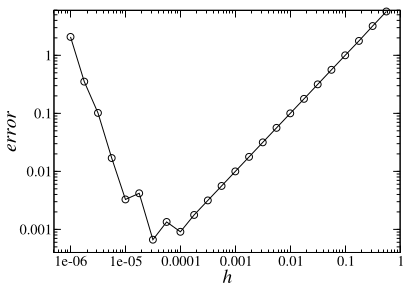
\includegraphics[width=0.8\linewidth]{img/errorh.png}
			\caption{errore di un metodo di Eulero $y_{n+1}=y_n+2hx_n$ in funzione di $h$, usato per integrare la funzione $y'=2x$ con condizione iniziale $y(0)=0$}
			\label{fig:errore1}
		\end{figure}
	\end{multicols}
	
	
	%
	%
	\vspace{1cm}
	\subsubsection{stabilità, radici caratteristiche, regioni di A-stabilità}
	Sia $\{y_i\}$ la soluzione numerica corrispondente ai punti della mesh
	$x_0, x_1, \dots, x_n$, con passo $h$.
	Il metodo è \emph{stabile} se per ogni perturbazione iniziale
	$|z_i - y_i| < \varepsilon$ per $i<p$, la differenza rimane limitata:
	\[
	|z_i - y_i| < C\varepsilon \qquad \text{per ogni } i\geq p .
	\]
	Il metodo \textbf{converge} se $y_i$ è tale che $Max_{i<p}|Y_i-y_i|\rightarrow 0$ se $h\rightarrow 0$ e vale anche $Max_{i>p}|Y_i-y_i|\rightarrow 0$, allora $y_i$ si dice convergere a $Y_i$.
	
	Un metodo \textbf{consistente} ($\sum_{j=0}^p a_j = 1$) \emph{è convergente se e solo se è stabile}.
	
	
	Il problema della stabilità è difficile, notiamo però che in generale integrare è un problema legato al trovare le radici di un polinomio, esprimiamo ancora il punto $y_{n+1}$ come combinazione lineare dei punti vicini e le derivate:
	
	\[ y_{n+1} = \sum^p_{j=0} a_j y_{n-j} + h\sum^p_{j=-1} b_j y'_{n-j}\ \ \ \ , \]
	
	dove in generale vale $\sum^p_{j=0} a_j = 1$ mentre $\sum^p_{j=0} ja_j = \sum^p_{j=-1} b_j$
	
	La stabilità e la convergenza sono assicurate dalla \emph{root condition}:
	
	\[ \rho(r) = r^{p+1} - \sum ^ p_{j=0}a_j r^{p-j} \]
	
	questo polinomio ha $p+1$ radici, notiamo inotre che $\rho(1)=0$ cioè 1 è sempre una radice. La condizione ci dice che:
	\begin{itemize}
		\item $|r_j|\leq 1$ per $j=0,1,\dots, p$
		\item $|r_j|=1$ se $r_j$ è una radice semplice
	\end{itemize}
	e - se soddisfatto - implica che il metodo sia stabile.
	Richiamiamo il generico \emph{multi-step} di eq.\ref{multistep}, in questo caso $p=1$ e $a_0=1$, le radici di $0=r^2-r$ sono 0 ed 1 quindi il metodo è stabile.
	
	Si ottengono condizioni più stringenti se si considera un'equazione differenziale test $y' = \lambda y(x)$, che ha soluzione di tipo se ci chiediamo le radici in questo caso abbiamo:
	
	\[ \color{blue}{\rho}\color{black}{^{n+1} = \sum^p_{j=0} a_j} \color{blue}{\rho}\color{black}{_{n-j} +} \color{blue}{\lambda} \color{black}h\sum^p_{j=-1} b_j \color{blue}{\rho}\color{black}_{n-j}\ \ \ \ ,\]
	
	da cui ricaveremmo $p+1$ radici $\rho_i(\lambda h)$:
	\begin{itemize}
		\item Il metodo è \textbf{relativamente stabile} se $|\rho_j(\lambda h) |\leq \rho_0(\lambda h)$ per $j=1,\dots, p$;
		\item Il metodo è \textbf{debolmente stabile} altrimenti.
	\end{itemize}
	
	Per il nostro multi-step : $a_0=1$, $b_0=3/2$, $b_1=-1/2$, $p=1$:
	
	\[ \rho^2 - (1+3\lambda h/2)\rho + \lambda h/2 = 0\ \ \ \ \ \  \Rightarrow \ \ \ \ \ \ \rho = \frac{1+3\lambda h/2 \pm \sqrt{(1+3\lambda h/2)^2-2\lambda h}}{2}\]
	
	\[\Rightarrow \ \ \ \ \rho_{0,1 }\sim  1+\lambda h, \ \ \frac{\lambda h}{2}\ \ \ \ \ \text{il metodo è relativamente stabile, ma } \lambda<0\]
	
	\begin{multicols}{2}
		Invece il metodo è \textbf{assolutamente stabile} se $|\rho_j(\lambda h)|<1$ per $j=0,1,\dots, p$. Nel caso del nostro multi-step abbiamo scritto sopra i valori e stavolta facciamo una considerazione senza approssimazione su 
		\[\rho_{0,1} = \frac{1+3\lambda h/2 \pm \sqrt{(1+3\lambda h/2)^2-2\lambda h}}{2}\ \ \ \ ,\]
		che è A-stabile per $-1<\lambda h< 0$
		
		\begin{figure}[H]
			\centering
			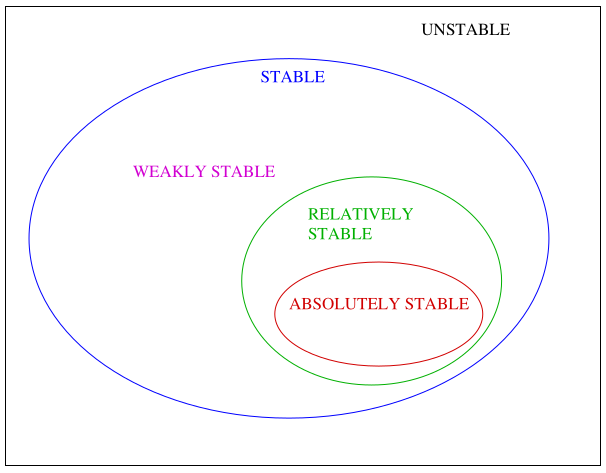
\includegraphics[width=0.7\linewidth]{img/venn.png}
			\caption{Schema visivo per comprendere i diversi tipi di stabilità}
			\label{fig:venn}
		\end{figure}
		
	\end{multicols}
	
	
	Per un metodo numerico, la soluzione approssimata soddisfa
	\[
	y_{n+1} = \rho(z)\, y_n, \qquad z = h\lambda,
	\]
	dove $\rho(z)$ è il fattore di amplificazione numerico. Una regione di stabilità è il luogo geometrico dei valori complessi $z=h\lambda$ per cui il metodo numerico NON amplifica errori quando la soluzione vera è smorzante, la \emph{regione di stabilità assoluta} è l'insieme dei valori $z \in \mathbb{C}$ tali che $|\rho(z)| < 1$.
	
	\begin{multicols}{2}
		La figura mostra un esempio regioni di stabilità:
		\begin{itemize}
			\item in rosso: i metodi Adams--Bashforth (AB), espliciti;
			\item in verde: i metodi Adams--Moulton (AM), impliciti.
		\end{itemize}
		Si osserva che i metodi AB hanno regioni di stabilità più piccole, mentre i metodi AM
		sono significativamente più stabili.
		
		\begin{figure}[H]
			\centering
			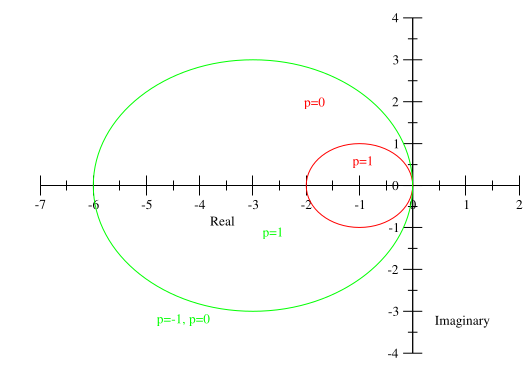
\includegraphics[width=\linewidth]{img/stability.png}
			\caption{Esempio di una regione di stabilità}
			\label{fig:placeholder}
		\end{figure}
	\end{multicols}
	
	
	%
	%
	\vspace{1cm}
	\subsubsection{Confronto di metodi multi-step}
	
	Guardiamo un primo confronto fra alcuni metodi che possiamo scrivere viste le cose affrontate:
	
	\begin{itemize}
		\item \textbf{metodo di Eulero}: $y_{n+1} = y_n + h y'_n + O(h^2)$, relativamente stabile;
		\item metodo del punto medio (\textbf{midpoint}): $y_{n+1}=y_{n-1} + 2 h y'_n + O(h^3)$, debolmente stabile;
		\item Adams-Bashforth (\textbf{AB(2)}): $y_{n+1}=y_n + h(3y'_n-y'_{n-1})/2 + O(h^3)$, assolutamente stabile;
		\item \textbf{metodo dei trapezi}: $y_{n+1}=y_n + h(y'_n-y'_{n+1})/2 + O(h^3)$, stabile, per $\lambda <0$ è assolutamente stabile.
	\end{itemize}
	
	\begin{multicols}{2}
		
		\begin{figure}[H]
			\centering
			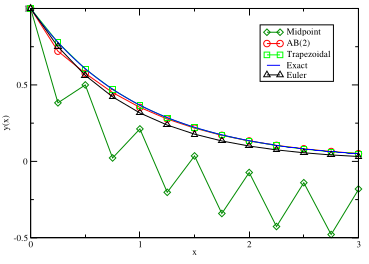
\includegraphics[width=7cm]{img/example.png}
			\caption{Integrazione di $y'=-y$ con h=0.25 e condizioni al contorno $y(0)=1$}
			\label{fig:example1}
		\end{figure}
		
		\begin{figure}[H]
			\centering
			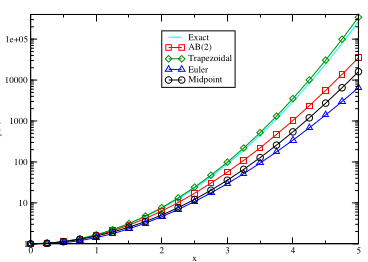
\includegraphics[width=7cm]{img/example2.png}
			\caption{Integrazione di $y'=xy$ con h=0.25 e condizioni al contorno $y(0)=1$}
			\label{fig:example1}
		\end{figure}
		
	\end{multicols}
	
	Eulero che è relativamente stabile e di ordine $h^2$ è da considerarsi migliore del midpoint che sarà anche di ordine $h^3$ ma è solamente debolmente stabile.
	Però, in un sistema già instabile - ad esempio $y'=xy$ in cui la soluzione è un esponenziale - conta invece solo l'ordine di errore.
	
	
	%
	%
	\vspace{1cm}
	\subsection{Metodi one-step}
	Nei metodi one-step, $y_{n+1}$ dipende unicamente da $y_n$, si capisce bene come il vantaggio più grande sia non dover tenere in memoria le $y_{n-j}$ che usavamo nei metodi multi-step.
	
	Il metodo one-step più banale è una comune espansione di Taylor della soluzione:
	\[
	y(t+h) = y(t) + hy'(t) + \frac{h^2}{2}y''(t) + \cdots,
	\]
	fermandosi alla derivata n-esima si ottiene un metodo numerico di ordine desiderato. Questo metodo non è generalmente utilizzato ma è molto facile da usare e appropriato quando la soluzione è di tipo polinomiale.
	
	Poiché $y' = f(t, y(t))$, la seconda derivata si ricava tramite la regola della catena:
	\[
	y'' \ =\ \frac{\partial}{\partial t}f(t,y) + \frac{\partial}{\partial y}f(t,y) \frac{\partial}{\partial y} y(t)
	\ =\ f_t(t,y) + f_y(t,y) f(t,y).
	\]
	
	Un metodo di Taylor del secondo ordine è quindi dato da:
	\[
	y_{n+1}
	= y_n
	+ h\, f(t_n, y_n)
	+ \frac{h^2}{2}
	\left[
	f_t(t_n,y_n)
	+ f_y(t_n,y_n) f(t_n,y_n)
	\right].
	\]
	
	In molti casi, metodi come il trapezoidale implicito o i metodi di Runge--Kutta
	permettono di raggiungere lo stesso ordine di accuratezza con un numero minore di derivate richieste.
	
	
	%
	%
	\subsubsection{metodi Runge-Kutta}
	
	L'idea dei metodi Runge-Kutta (RK) è quella di approssimare l'integrale
	\[
	y(t+h) = y(t) + \int_{t}^{t+h} f(\tau, y(\tau))\, d\tau,
	\]
	costruendo una stima accurata della pendenza media della soluzione nel tratto
	$[t, t+h]$. A differenza dei metodi multistep, i metodi RK utilizzano soltanto
	le informazioni al punto $(t,y)$ corrente, senza ricorrere ai valori precedenti.
	%
	Per comprendere come si arriva a tali schemi, possiamo ricostruire passo per passo 
	la procedura intuitiva che porta dapprima a un metodo di ordine due (RK2) e poi
	al classico metodo di ordine quattro (RK4).
	%
	
	\begin{multicols}{2}
		
		Prendiamo ad esempio la funzione $y(x)$ soluzione dell'ODE $y'=f(x, \, y(x))=2\sqrt{-y}$ con condizione iniziale $y(0)=-1$, costruiamo l'approssimazione supponendo di essere arrivati ad integrare fino ad un punto $x_0$ e vogliamo proseguire di $h$:
		\begin{enumerate}
			\item come prima cosa si calcola la derivata nel punto $x_0$, $y'(x_0) = f(x, \, y(x))_{|x=x_0}$, come si vede in verde in figura;
			\item ci si sposta di $\color{green}{k_1} \color{black}= h f(t,\, y)$ arrivando nel punto di ascissa $x_f=x_0+h$ ma non lungo la soluzione poichè si è proseguiti linearmente lungo la retta verde, qui si calcola $\color{magenta}{k_2} \color{black}= h f(t_n + h,\,  y_n + \color{green}{k_1} \color{black})$, come si vede in magenta in figura;
			\item si prende la media dei due spostamenti sulle ordinate $k_1$ e $k_2$:
			\[\boxed{y_{n+1} = y_n + \frac{\color{green}{k_1} \color{black}{+} \color{magenta}{k_2}}{2}} \ \ .\]
		\end{enumerate}
		
		
		\begin{figure}[H]
			\centering
			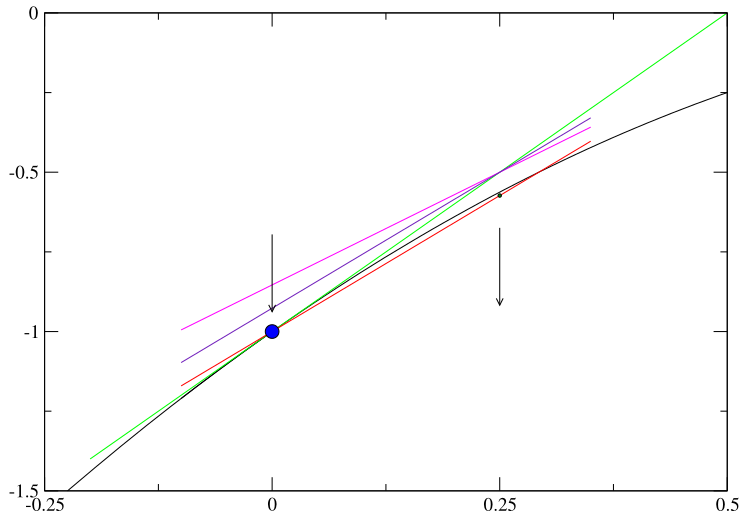
\includegraphics[width=\linewidth]{img/example_RK.png}
			\caption{esempio visuale di applicazione di Runge-Kutta}
			\label{fig:placeholder}
		\end{figure}
		
	\end{multicols}
	
	I passaggi spiegati sono la base del Runge-Kutta e corrispondono ad un metodo del secondo ordine.
	
	Per ottenere ordini superiori, si introducono valutazioni intermedie della derivata. L'idea è approssimare sempre meglio il valore della pendenza media integrale, scegliendo opportunamente ascisse intermedie e combinazioni lineari delle derivate.
	
	\begin{multicols}{2}
		Un metodo RK di ordine quattro può utilizzare quattro valutazioni:
		\[
		\begin{aligned}
			k_1 &= h f(t_n, y_n), \\ 
			\\
			k_2 &= h f\bigl(t_n + \tfrac{h}{2},\, y_n + \tfrac{k_1}{2}\bigr), \\ \\
			k_3 &= h f\bigl(t_n + \tfrac{h}{2},\, y_n + \tfrac{k_2}{2}\bigr), \\ \\
			k_4 &= h f(t_n + h,\, y_n + k_3).
		\end{aligned}
		\]
		
		\begin{figure}[H]
			\centering
			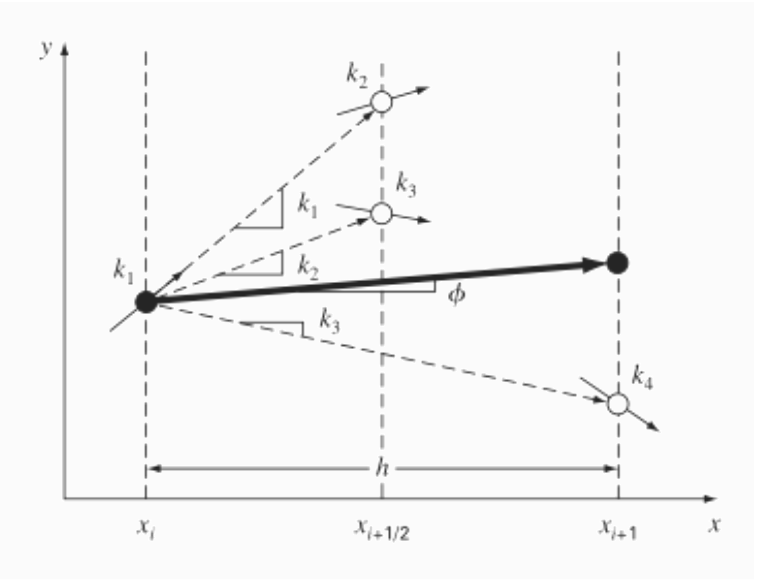
\includegraphics[width=0.8\linewidth]{img/rk4.png}
			\caption{Visualizzazione delle 4 valutazioni da fare in un RK4}
			\label{fig:RK4}
		\end{figure}
		
	\end{multicols}
	Ogni $k_i$ è una stima della derivata in un punto diverso dell'intervallo, costruita per compensare l'errore di espansione di Taylor del passo precedente.
	l valore numerico della soluzione viene aggiornato combinando i contributi:
	
	\begin{equation}\label{eq:Runge-Kutta 4}
		\boxed{y_{n+1} = y_n + \frac{1}{6}
			\bigl(k_1 + 2k_2 + 2k_3 + k_4\bigr)}\ \ \ .
	\end{equation}
	
	Questa particolare combinazione lineare è scelta in modo che l'errore globale
	sia dell'ordine $h^4$, e che l'espansione in serie di Taylor del metodo
	coincida con quella della soluzione esatta fino ai termini di ordine $h^4$.
	Il metodo risultante è il molto utilizzato \emph{Runge--Kutta del quarto ordine} (\textbf{RK4}).
	
	\begin{dimostrazione}{}
		Ricorda le parole del Mannella: Runge-Kutta va usato con passo temporale variabile, a passo fisso fa schifo!
	\end{dimostrazione}
	
	
	\subsubsection{Controllo del passo mediante Richardson}
	
	Una tecnica classica per stimare l'errore locale di un metodo one-step consiste
	nell'applicare lo stesso algoritmo con due passi diversi, $h$ e $2h$, e
	confrontare i risultati.  
	Sia $Y(x_n)$ la soluzione esatta e $y_h(x_n)$ l'approssimazione ottenuta con passo $h$ e $y_{2h}(x_n)$ quella
	ottenuta con passo $2h$.  
	Per un metodo di ordine due (come il trapezoidale), vale lo sviluppo:
	
	\[
	Y(x_n) - y_h(x_n) = D(x_n) h^2 + O(h^3),
	\qquad
	Y(x_n) - y_{2h}(x_n) = 4 D(x_n) h^2 + O(h^3).
	\]
	Eliminando il coefficiente ignoto $D(x_n)$ si ottiene un'approssimazione più precisa:
	\[
	Y(x_n)\ \approx \ \frac{4 y_h(x_n) - y_{2h}(x_n)}{3} + O(h^3)\ \ ,
	\]
	quindi una stima dell'errore è data da:
	\[
	Y(x_n) - y_h(x_n)\  \approx \ 
	\frac{y_h(x_n) - y_{2h}(x_n)}{3} \ \ .
	\]
	Questa informazione permette di regolare dinamicamente il passo di integrazione
	per mantenere l'errore entro una tolleranza prefissata. 
	L'unico limite pratico è che, per stimare l'errore, occorre disporre sia
	dell'integrazione a passo $h$ sia di quella a passo $2h$.
	
	\begin{table}[H]
		\centering
		\begin{tabular}{c|c|c|c|c}
			\hline
			$x$ & $y_h(x)$ & $y_{2h}(x)$ & Errore stimato & $Y(x)-y_h(x)$ \\
			\hline
			1.0 & 0.49602 & 0.48314 & 0.00429 & 0.00398 \\
			2.0 & 0.33099 & 0.32361 & 0.00246 & 0.00234 \\
			3.0 & 0.24852 & 0.24389 & 0.00154 & 0.00148 \\
			4.0 & 0.19899 & 0.19484 & 0.00105 & 0.00101 \\
			5.0 & 0.16594 & 0.16366 & 0.00076 & 0.00073 \\
			\hline
		\end{tabular}
		\caption{Stima dell'errore tramite Richardson (Atkinson, $y'=-y^2$, $y(0)=1$, $h=0.25$).}
	\end{table}
	
	
	
	%
	%
	\subsubsection{Il metodo del midpoint modificato}
	
	Il metodo del midpoint modificato è un algoritmo one-step composto che
	permette di muovere la soluzione da $x$ a $x+H$ suddividendo l'intervallo in
	$n$ sotto-passi di ampiezza $h = H/n$.  
	Si introducono le variabili ausiliarie $z_m$, con:
	\[
	z_0 = y(x), \qquad
	z_1 = z_0 + h f(x, z_0),
	\]
	e la ricorrenza centrale:
	\[
	z_{m+1} = z_{m-1} + 2h\, f(x + m h, z_m),
	\qquad m = 1,2,\dots,n-1.
	\]
	Il valore finale è ottenuto tramite:
	\[
	y(x+H) \approx y_n =
	\frac{1}{2}\bigl(z_n + z_{n-1} + h f(x+H,\, z_n)\bigr).
	\]
	
	L'aspetto notevole di questo metodo è che l'errore dipende soltanto da potenze
	pari di $h$, cioè:
	\[
	y(x+H) - y_n = \sum_{k=1}^{\infty} \alpha_k h^{2k}.
	\]
	Questa proprietà lo rende particolarmente adatto all'accoppiamento con metodi
	di estrapolazione, riducendo drasticamente il numero di valutazioni della
	funzione richiesta per ottenere alta accuratezza.
	
	
	%
	%
	\subsubsection{Richardson extrapolation e metodo di Burlisch--Stoer}
	
	\begin{multicols}{2}
		La \emph{Richardson extrapolation} si basa sull'idea che l'approssimazione ottenuta
		da un metodo one-step su un intervallo di ampiezza $H$ dipende analiticamente
		dal passo elementare $h = H/n$.  
		Applicando l'algoritmo elementare con $n = 1, 2, 4, 8, \dots$ sotto-passi,
		si ottengono approssimazioni $y_1, y_2, y_4, y_8, \dots$, che possono essere
		estrapolate nel limite $n \to \infty$ (ossia $h \to 0$) utilizzando una
		funzione razionale
		
		\begin{figure}[H]
			\centering
			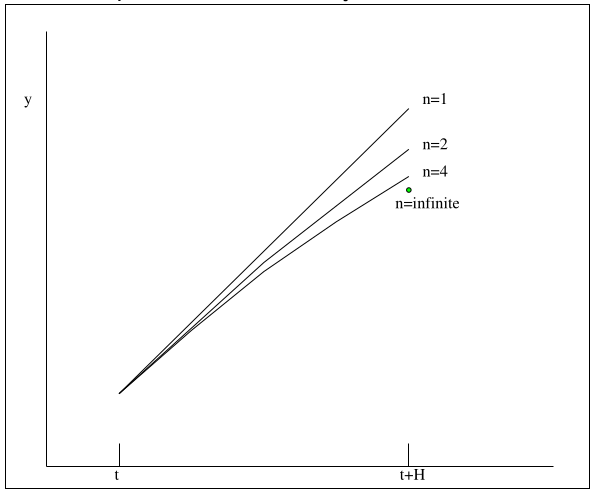
\includegraphics[width=0.8\linewidth]{img/richardson-extr.png}
			\caption{Idea dietro l'estrapolazione di Richardson}
			\label{fig:richardson}
		\end{figure}
	\end{multicols}
	
	\[
	\boxed{R_{i(i+1)\dots (i+m)} = 
		\frac{p_0 + p_1 x + \cdots + p_\mu x^\mu}
		{1 + q_1 x + \cdots + q_\nu x^\nu}} \ ,
	\qquad x = \frac{H}{n}.
	\]
	
	Questo è il risultato del \textbf{metodo di Burlisch-Stoer} che combina queste due idee:
	
	\begin{enumerate}
		\item usa il \emph{midpoint modificato} come metodo elementare di integrazione
		su $[x, x+H]$;
		\item applica la Richardson extrapolation ai risultati ottenuti per
		$n = 1,2,4,\dots$;
		\item costruisce una matrice di estrapolazione (tabella di Richardson)
		da cui selezionare la stima più accurata.
	\end{enumerate}
	
	La scelta del passo $H$ e del numero di sotto-passaggi $n$ è adattata dinamicamente
	per minimizzare il costo computazionale mantenendo al contempo l'errore entro
	limiti prestabiliti.  
	Il metodo Burlisch--Stoer è estremamente efficiente per funzioni sufficientemente
	regolari ed è in grado di raggiungere ordini molto elevati, pur senza ricorrere
	a valutazioni multiple di derivate alte.
	
	
	%
	%
	\vspace{1cm}
	\subsubsection{Metodi Runge-Kutta Hamiltoniani}
	
	Consideriamo un sistema Hamiltoniano del tipo: $\boxed{H(q,p) = \displaystyle\frac{p^2}{2} + V(q)}$, con equazioni del moto:
	\[
	\dot{q} = \frac{\partial H}{\partial p}\, , \qquad
	\dot{p} = -\frac{\partial H}{\partial q}\, ,
	\]
	e date certe condizioni al contorno $p(0)$ and $q(0)$. Vista la forma di RK4 pensiamo di potervi costruire una \emph{contact transformation}, ovvero una mappa da $q,\, p$ a $Q,\, P$ dove questi ultimi possono essere pensati come un evoluzione a un tempo successivo di $q,\, p$.
	
	
	L'evoluzione generata da tali equazioni è una trasformazione \emph{simplettica},
	cioè preserva la struttura geometrica del flusso Hamiltoniano, come le trasformazioni canoniche studiate a meccanica classica (vedi capitolo settimo di '\emph{Fisica teorica I: meccanica}' di Landau-Lif\v{s}its). 
	
	I metodi numerici come i Runge-Kutta classici, non sono in generale
	simplettici e possono introdurre deriva energetica nelle integrazioni di lungo periodo.
	
	\paragraph{Idea generale.}
	Un metodo Runge--Kutta Hamiltoniano (o simplettico) cerca di costruire una mappa
	\[
	(q_n,p_n) \longmapsto (q_{n+1},p_{n+1})
	\]
	che sia a sua volta una trasformazione simplettica e che approssimi il flusso
	esatto dopo un passo $h$.
	
	Per un metodo RK con coefficienti $\{a_i,b_i\}$, la trasformazione RK simplettica di ordine $n$ assume la forma:
	\[
	p_{j} = p_{j-1} + h b_j\, F(q_{j-1}), \qquad
	q_{j} = q_{j-1} + h a_j\, p_j,
	\]
	che non sono nient'altro che l'implementazione delle equazioni di Hamilton, dove $F(q) = -V'(q)$ e ricordiamo di avere delle condizioni iniziali $p_0$, $q_0$ con cui andiamo a valutare $p_n$, $q_n$ come punti evoluti dopo un tempo h, l'aggiornamento 'sfalsato' per cui $p_{j}$ dipende dai $p_{j-1},\, q_{j-1}$ precedenti ma $q_j$ dipende da $q_{j-1},\, p_j$  serve a mantenere la simpletticità.
	
	\paragraph{\emph{'Velocity Verlet'} / \emph{'Leapfrog'}}
	L'esempio più semplice è quello in cui prendiamo la forma appena scritta per $q_1$, $p_1$, $q_2$, $p_ancora2$ ed inseriamo i coefficienti $a_1=a_2=\frac{1}{2}$, $b_1=0$, $b_2=1$:
	\[p_1\ =\ p_0 + h \times 0 \times F(q_0)\ =\ p_0\]
	\[q_1\ =\ q_0 + h\times \frac{1}{2} \times p_1\ =\ q_0 + \frac{h}{2}p_1\]
	\[p_2\ =\ p_1 + h \times 1 \times F(q_1)\ =\ p_0 + hF(q_1) \]
	\[q_2\ =\ q_1 + h\times \frac{1}{2} \times p_2\ =\ q_1 + \frac{h}{2}p_2\]
	
	Interpretazione: $q$ avanza in due metà simmetriche ($a_1=a_2=\frac{1}{2}$), mentre la $p$ viene aggiornata solo a seguito di un mezzo passo in avanti.
	
	
	\paragraph{Esempio di schema simplettico.}
	Una scelta possibile di coefficienti \emph{magici} è:
	\[
	\begin{array}{c|c}
		i & (a_i, b_i) \\
		\hline
		1 & \left(0.515352837431123,\; 0.134496199277431\right)\\
		2 & \left(-0.085782019412974,\; -0.224819803079421\right)\\
		3 & \left(0.441583023616467,\; 0.756320000515668\right)\\
		4 & \left(0.128846158365384,\; 0.334003603286321\right)
	\end{array}
	\]
	
	\paragraph{Esempio pratico.}
	Per il sistema $H(q,p) = \frac{p^2}{2} + \frac{q^4}{4} - \frac{q^2}{2}$,
	la comparazione tra un RK standard e un RK Hamiltoniano mostra che il metodo
	simplettico conserva l'Hamiltoniana in modo molto più accurato nel tempo,
	evitando il drift energetico tipico dei metodi non-simplettici.
	
	
	%
	%
	\vspace{0.5cm}
	\subsection{Equazioni stiff}
	
	Un'equazione differenziale si dice \href{https://en.wikipedia.org/wiki/Stiff_equation}{\emph{stiff}} quando presenta scale temporali
	molto diverse: la soluzione varia lentamente su larga scala, ma la dinamica
	interna dell'equazione contiene componenti che decadono estremamente velocemente.
	In questi casi, i metodi espliciti richiedono passi $h$ molto piccoli per
	ragioni di stabilità, anche quando la soluzione vera non lo richiederebbe.
	
	\paragraph{Esempio semplice.}
	Immaginiamo di dover risolvere un problema come un sistema 
	\[
	\begin{cases}
		u'(x) = 998\, u(x) + 1998\, v(x)\,, \quad \quad u(0)=1\\
		v'(x) = -999\, u(x) - 1999\, v(x)\,, \quad \quad v(0)=0
	\end{cases}
	\]
	Si può notare che le soluzioni analitiche esistono e sono $u(x)=2e^{-x}-e^{-1000x}$ e $v(x)=-e^{-x}+e^{-1000x}$, ma dovendo risolvere tramite metodi numerici finiremmo per usare time step troppo piccoli per sopperire alla presenza di modi con tempi scala molto lontani fra loro, lo si vede subito scrivendo la matrice del sistema 
	
	\[
	A = \begin{pmatrix}
		998 & 1998 \\
		-999 & -1999
	\end{pmatrix}
	\quad \quad \quad \quad \lambda_{1,\, 2}\, =\, -1,\, -1000
	\]
	
	\paragraph{Come affrontare il problema?}
	
	Affrontiamo il problema grazie a metodi impliciti/semi-impliciti ad ordine basso, in particolare presa $y'=f(x,\, y(x))$, si linearizza un metodo di Euler implicito:
	
	\[ y_{n+1}\ =\ y_n\, +\, h\, \color{blue}{f(x_{n+1},\, y_{n+1})}\]
	\[ y_{n+1}\ =\ y_n\, +\, h\left[ \color{blue}{ f(x_{n+1},\, y_n) \, +\, \frac{\partial
			f}{\partial y_n} (y_{n+1} - y_n)} \color{black}\right] \]
	Portando a sinistra il termine con $y_{n+1}$ e dividendo i due membri rimane:
	\[ y_{n+1}\ =\ \left[  1-h\, \frac{\partial
		f}{\partial y_n}  \right]^{-1}\, \left( y_n + h\, f(x_{n+1}, y_{n} ) - h\, \frac{\partial f}{\partial y_n} y_n \right)\]
	
	
	Formalmente, definita $\textbf{A}$ la matrice del nostro sistema lineare (matrice definita positiva, $\lambda_i > 0 \, \, \forall\,  i$) e dato $\textbf{y}'=-\textbf{A}\, \textbf{y}$, utilizzando un metodo di eulero esplicito abbiamo:
	
	\[ \textbf{y}_{n+1}\ =\ \textbf{y}_n + h\textbf{y'}_n\ =\  ( 1 - h\, \textbf{A} )\, \textbf{y}_n\ \equiv\ \textbf{B}\, \textbf{y}_n \]
	
	e $\textbf{B}^n\rightarrow 0$ per $n\rightarrow \infty$ solo se gli autovalori $(1-\lambda_i h)\equiv \mu_i$ di \textbf{B} sono $<1$ e questo tipicamente non accade per le \emph{stiff equations}.
	
	Tuttavia, usando un metodo implicito che assume la forma $\boxed{(Id + h\textbf{A}) \textbf{y}_{n+1} = \textbf{y}_n}$ da non confondere con il metodo esplicito appena sviluppato sopra, abbiamo una diversa \textbf{B}: $\textbf{y}_{n+1} = (Id + h\textbf{A})^{-1}\textbf{y}_n\equiv \textbf{B} \textbf{y}_n$.
	Se gli autovalori di \textbf{A} sono $\lambda>0$, allora gli autovalori di $(Id+h\textbf{A})^{-1}$ sono $\mu_i\equiv(1+h\lambda)^{-1}\, \, \forall\, h$ quindi la soluzione si comporta bene ($0<\mu_i<1$).
	
	
	
	
	%
	%
	\vspace{0.5cm}
	\subsection{Boundary Value Problems (BVP)}
	
	Prendiamo di esempio un'equazione di un oscillatore armonico smorzato $y''=-\gamma y' -\omega_0^2 y$ con una condizione iniziale $y(0)=1$ ed un'altra condizione al tempo finale $t_f=k\pi/\omega$, dove $\omega^2 \equiv \omega^2_0-\gamma^2/4$.
	
	Il problema che si verifica è che data la tipica soluzione $y(t)=e^{-\gamma t/2}(A\,sin(\omega t)+B\,cos(\omega t))$, mentre la condizione iniziale ci porta ad imporre $A=0$, la condizione sul punto finale non porta alcuna informazione in più per B perché abbiamo scelto il punto finale in un nodo dell'oscillazione portandoci ad avere $y(t_f)=e^{-\gamma t/2} (-1)^k$ che non contiene né B né A quindi non ci aiuta a trovare una soluzione univoca.
	
	Abbiamo quindi un grosso problema: \emph{la soluzione non è unica!}
	
	Vediamo due diversi modi per affrontare il problema.
	
	\subsubsection{Shooting method}
	Come si può immaginare dal nome, qui \emph{spariamo} a caso.
	
	Ripartiamo dallo stesso problema di oscillatore armonico smorzato e immaginiamo di voler imporre la condizione al tempo finale $y(t_f)=y(5.02)=0.418$.
	
	Diamo dei valori alle costanti, come $\gamma=0.3$ ed $\omega_0=1$, a questo punto siamo costretti per costruire una simil-soluzione a imporre un'altra condizione iniziale, come la derivata $y'(0)=s$, fatto ciò integriamo fino al punto finale.
	
	Ripetiamo la costruzione per diversi valori di $s$ fino ad averne uno che approssimi bene la condizione che avremmo voluto imporre: $y(5.02,\, s)\approx0.418$.
	
	\subsubsection{metodo di rilassamento / differenze finite}
	
	Il metodo consiste nel mettere un tentativo di soluzione, \emph{initial guess}, fra $x_0$ ed $x_f$ e 'rilassarlo' fino a trovare la soluzione corretta.
	
	Partiamo ad esempio da una $y''=f(x, y, y')$ con condizioni al bordo $y(x_0)=g_0$ e $y(x_n)=g_n$. Si assume una mesh di n punti spaziati di un passo $h$, usando le formule delle differenze finite possiamo scrivere:
	
	\[
	\frac{y_{n-1}-2y_n + y_{n+1}}{h^2}\ =\ f(x_n,\, y_n,\, \frac{y_{n+1}-y_{n-1}}{2h})\  \equiv\ f_n
	\]
	
	dove $y_0$ e $y_n$ sono condizioni date in precedenza, riscriviamo in forma matriciale il problema:
	
	\[ \frac{1}{h^2}
	\begin{pmatrix}
		-2 & 1 & 0 & \cdots & 0 \\
		1 & -2 & 1 & \cdots & 0 \\
		0 & 1 & \ddots & \ddots & \vdots \\
		\vdots & \ddots & \ddots & -2 & 1 \\
		0 & \cdots & 0 & 1 & -2
	\end{pmatrix}
	\begin{pmatrix}
		y_1 \\ y_2 \\ y_3 \\ \vdots \\ y_{n-1}
	\end{pmatrix}
	\ =\ \begin{pmatrix}
		f_1 \\ f_2 \\ \vdots \\ \\ f_{N-1}
	\end{pmatrix} - \begin{pmatrix}
		g_0/h^2 \\ 0 \\ \vdots \\ 0\\ g_{n}/h^2
	\end{pmatrix}
	\]
	
	che può essere scritto come $\displaystyle\frac{1}{h^2} \textbf{A}Y \equiv \textbf{F}(Y) + \textbf{G}$ e da questa forma si risolve con metodo di Newton dopo aver linearizzato F(Y):
	
	\[
	\textbf{y}^{(m+1)}\ =\ \textbf{y}^{(m)}\ -\ \left[ \frac{\textbf{A}}{h^2} - \frac{\partial \textbf{F}_i}{\partial y_j} \right]^{-1}\, \left[ \frac{\textbf{A}y^{m}}{h^2} - \textbf{F}(y^{(m)}) - \textbf{G} \right]
	\]
	
	A questo punto possiamo dare un guess iniziale $y^{(0)} $ ed iterare.
	
	
	
	%
	%
	\newpage
	\section{Equazioni differenziali alle derivate parziali (PDE)}
	Esistono principalmente tre tipi di equazioni differenziali alle derivate parziali (PDE, \emph{partial differential equation}), la differenza computazionalmente sta nel caso in cui abbiamo \textbf{valori iniziali} (problema principale: stabilità) o utilizziamo \textbf{condizioni al contorno} (problema principale: efficienza):
	\begin{itemize}
		\item \textbf{Iperboliche}: come ad esempio l'equazione delle onde 
		\begin{equation}
			\boxed{\frac{\partial^2 u}{\partial t^2} - v^2 \frac{\partial^2 u}{\partial x^2}\ =\ 0}\ \ \ \ ; 
		\end{equation}
		\item \textbf{Paraboliche}: come ad esempio l'equazione di diffusione 
		\begin{equation}
			\boxed{\frac{\partial P}{\partial t} - \frac{\partial}{\partial x}\left( D\frac{\partial }{\partial x}P\right) \ =\ 0}\ \ \ \ ; 
		\end{equation}
		\item \textbf{Ellittiche}: come ad esempio l'equazione di Poisson 
		\begin{equation}
			\boxed{\frac{\partial^2 u}{\partial x^2} +  \frac{\partial^2 u}{\partial y^2}\ =\ \rho(x, y)}\ \ \ \ .  
		\end{equation}
	\end{itemize}
	
	\begin{dimostrazione}{applicazione}
		Mettiamo che io prenda $\displaystyle\frac{\partial^2 u}{\partial x^2} +  \frac{\partial^2 u}{\partial y^2} = \rho(x, y)$, prima cosa che vorremmo fare è introdurre uno \emph{spacing} $\Delta$ in modo che ${x_j}=x_0+j\Delta$ (con j=0, ..., J) e ${y_\ell}=y_0+j\Delta$ (con $\ell$=0, ..., L).\\
		Possiamo esprimere le derivate come spiegato nel paragrafo sulle differenze finite:
		\[\frac{u_{j+1,\ \ell}-2u_{j,\ \ell} + u_{j-1,\ \ell}}{\Delta^2} + \frac{u_{j,\ \ell+1}-2u_{j,\ \ell} + u_{j,\ \ell-1}}{\Delta^2}\ =\ \rho(x, y)\]
		Il modo di soluzione che introduciamo ora passa attraverso l'introdurre un indice $i=j(L+1)+\ell$ (per j=0 va da 0 ad L, per j=1 va da L+1 a 2L+1 e così via...) così che u diventi un vettore ed il problema diventi un problema di algebra lineare:
		\[ u_{i+L+1}+u_{i-(L+1)} + u_{i+1} + u_{i-1} - 4u_i \ =\ \Delta^2 \rho(x, y)\ \ \ \ ,\]
		\[ \textbf{A}\ \vec u\ = \ \vec b \]
		
		dove in questo caso ci si può convincere che 
		\[\textbf{A}=\left[
		\begin{array}{ccc|ccc|ccc}
			-4 & 1 &  & 1 & &  &  &  &  \\
			1 & -4 & 1 &  & 1 &  &  &  & \\
			& 1 & -4 &  &  & 1 &  &  &  \\
			\hline
			1 &  &  & -4 & 1 &  & 1 &  &  \\
			& 1 &  & 1 & -4 & 1 &  & 1 &  \\
			&  & 1 &  & 1 & -4 &  &  & 1 \\
			\hline
			&  & & 1 &  &  & -4 & 1 &  \\
			&  & & & 1 &  & 1 & -4 & 1 \\
			& & & & & 1 & & 1 & -4 \\
		\end{array}
		\right]
		\]
		
		
		Come risolvere $\textbf{A}\vec u = \vec b$? 
		\begin{itemize}
			\item quando \textbf{A} è costante con Fast Fourier methods;
			\item direttamente, usando ad esempio il gradiente coniugato (molto accurato, non molto efficiente quando \textbf{A} è grande perché 'sparsa');
			\item Rilassamento, scrivendo $\textbf{A}=\textbf{E}-\textbf{F}$ dove \textbf{E} è invertibile, si inizia da un guess $\vec u^{0}$ e si itera risolvendo $\textbf{E} \vec{u}^{(r+1)}=\vec b + \textbf{F} \vec u^{(r)}$
		\end{itemize}
	\end{dimostrazione}
	
	
	%
	%
	\vspace{1cm}
	\subsection{Differenze finite}
	
	Il metodo delle differenze finite è una strategia utilizzata per risolvere numericamente equazioni differenziali che, nelle sue varianti, si basa sull'approssimazione delle derivate con equazioni alle differenze finite. Viene utilizzato prevalentemente per equazioni differenziali ordinarie, anche se il metodo viene sfruttato come schema di avanzamento nel tempo per problemi alle derivate parziali.
	
	\[ u_{i+1}=u_i + u_i'dx + \frac{1}{2}u_i''dx^2 + ...  \]
	\[ \frac{u_{i+1}-u_i}{dx}= u_i' + \frac{1}{2}u_i''dx + ...  \]
	\[ u_{i+1}-u_{i-1} = 2u_i' dx + \frac{1}{6} u_i'''dx^3 \]
	
	Che cosa vuol dire? che la derivata nel punto i-esimo può essere in qualche modo ricavata attraverso valori della funzione u in i e nei punti vicini i+1, i-1, etc. .\\
	Possiamo poi stimare l'errore di queste stime grazie alle serie di Taylor.\\
	
	\[ u_{i=0}^{'} = \frac{1}{2dx} \left(- u_{-1} +u_1 \right) + ...dx^2 u_0^{'''}\ \ \ \ \ \ \ \ \ \ u_{0}^{'} = \frac{1}{12dx} \left[ u_{-2} - 8u_{-1} -  8u_1 - u_2\right]+ ...dx^4u_0^{(5)} \]
	\[ \text{con al bordo:}\ \ \ \ u^{'}_{0} = \frac{1}{dx} \left( -u_{0}+u_{1} \right) \ \ \ \ \text{oppure} \ \ \ \ \ u^{'}_{0}=\frac{1}{2dx} (-3u_0 + 4u_1 - u_2) \]
	
	\[ u_{0}^{''} = \frac{1}{dx^2} \left(u_{-1} -2u_0 + u_1 \right) + ...dx^2 u_0^{(4)}\ \ \ \ \ \ \ \ \ \ u_{0}^{''} = \frac{1}{12dx^2} \left( -u_{-2} +16u_{-1} -30u_0 + 16u_1 -u_2\right) + ...dx^2y_0^{(6)} \]
	\[ \text{con al bordo:}\ \ \ \  u^{''}_{0}=\frac{1}{dx^2} (-2u_0 -5u_{1}+4 u_2-u_3) \]
	
	
	
	%
	%
	\vspace{1cm}
	\subsection{Flux-conservative PDEs}
	Molte equazioni differenziali sono nella forma di un'equazione che conserva il flusso:
	\begin{equation}
		\boxed{\frac{\partial}{\partial t}\textbf{u}\ =\ -\ \frac{\partial}{\partial x}\textbf{F}(\textbf{u})}\ \ \ \ ,
	\end{equation}
	
	dove $\textbf{F}(u)$ è il flusso della quantità.\\
	Ad esempio, anche l'equazione standard iperbolica $\displaystyle \frac{\partial^2 u}{\partial t^2} = v^2 \frac{\partial^2 u}{\partial x^2}$ può essere scritta, definendo $s\equiv\frac{\partial}{\partial t}u$ e $r\equiv v \frac{\partial}{\partial x}u$, come un'equazione del tipo sopra definito:
	\[ \frac{\partial}{\partial t}s = v\frac{\partial}{\partial x}r \ \ \ ,\ \ \ \ \ \ \ \ \ \ \ \ \ \ \ \ \  \frac{\partial}{\partial t}r = v\frac{\partial}{\partial x}s\ \ \ \ \ \ , \]
	definendo $s\equiv\frac{\partial}{\partial t}u$ e $r\equiv v \frac{\partial}{\partial x}u$.\\
	
	
	%
	%
	\vspace{1cm}
	\subsubsection{Forward Time, Centered Space}
	Altro esempio di PDS che possiamo scrivere in forma flux-conservative è $\boxed{\displaystyle \frac{\partial u}{\partial t} = v \frac{\partial u}{\partial x}}$ se considerato $\textbf{F}(u)=vu$.
	Prendiamo appunto $\displaystyle \frac{\partial u}{\partial t} = v \frac{\partial u}{\partial x}$, usando $x_j=x_0+j\Delta x$ (j=0, ..., J) e $t_n=t_0+n\Delta t$ (n=0, ..., N) andiamo a discretizzare $u^n_j \equiv u(t_n, x_j)$ e ancora una volta esprimiamo le derivate a meno di un errore:
	\[\frac{\partial u}{\partial t}|_{j, n} = \frac{u_j^{n+1} - u_j^{n}}{\Delta t} + O(\Delta t)\ \ \ \ \ \ \ \ \ \ \ \ \ \ \ \ \ \frac{\partial u}{\partial x}|_{j, n} = \frac{u_{j+1}^{n} - u_{j-1}^{n}}{2\Delta x} + O(\Delta x^2)\]
	\begin{equation}\label{5}
		\frac{u_j^{n+1} - u_j^{n}}{\Delta t} = -v\left(\ \frac{u_{j+1}^{n} - u_{j-1}^{n}}{2\Delta x}\right)
	\end{equation}
	A partire da eq.\ref{5} sviluppiamo la soluzione chiamata \emph{forward time centered space} (\textbf{FTCS}), forma esplicita in cui esprimiamo i valori 'forward' $u^{n+1}$ nel tempo in funzione di $u^{n}$ e centrata nello spazio:
	\begin{equation}\label{Burgers FTCS}
		u^{n+1}_j = u^n_j - v \Delta t \frac{u_{j+1}^{n} - u_{j-1}^{n}}{2\Delta x}\ \ \ \ .
	\end{equation}
	Possiamo fare un'\textbf{analisi di stabilità di Von Neumann} arrivati a questo punto: l'idea è quella di studiare la stabilità lineare di un'onda, assumendo $u^n_j = e^{i(kx-\omega t)}$ e definito $\xi\equiv e^{i\omega \Delta t}$ si ha $\displaystyle u^n_j=\xi^n e^{ikj\Delta x}$ dove $\xi^n$ rappresenta l'ampiezza al tempo $t_n$.\\
	Sostituendo $u^n_j$ in eq.\ref{Burgers FTCS} si ottiene:
	\[\xi = 1+ i \frac{v\Delta t }{\Delta x} sin(k\Delta x)\ \ \ .\]
	Risulta chiaro che $|\xi|>1$ quindi secondo quest'analisi per ogni scelta di $\Delta x$ e $\Delta t$ il metodo è instabile $\forall$ k.
	
	
	
	%
	%
	\vspace{1cm}
	\subsubsection{Metodo di Lax}
	
	\begin{multicols}{2}
		Il metodo di Lax consiste nel sostituire $u^n_j\rightarrow \frac{u^n_{j+1}-u^n_{j-1}}{2}$ all'interno di eq.\ref{Burgers FTCS} così da fare un'analisi di stabilità di Von Neumann sulla forma:
		\[  u^{n+1}_j = \frac{u^n_{j+1}-u^n_{j-1}}{2} + v \Delta t \frac{u_{j+1}^{n} - u_{j-1}^{n}}{2\Delta x}\ \ \ \ .\]
		\[ \xi = cos(k\Delta x) - i \frac{v\Delta t}{\Delta x} sin (k\Delta x)\]
		dove abbiamo usato ancora $\displaystyle u^n_j=\xi^n e^{ikj\Delta x}$.\\
		\begin{figure}[H]
			\centering
			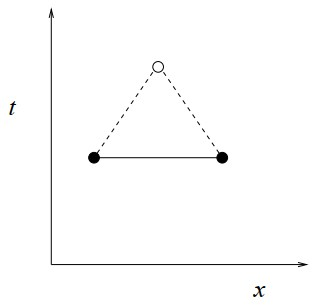
\includegraphics[width=0.5\linewidth]{img/LAX.jpg}
			\caption{Caption}
			\label{fig:placeholder}
		\end{figure}
	\end{multicols}
	Ora per la stabilità si ottiene $|\xi|^2 = cos^2(k\Delta x)+  \left( \frac{v\Delta t }{\Delta x}\right)^2 sin^2(k\Delta x)$, che può essere stabile ($|\xi|<1$) se viene rispettato il vincolo $\frac{|v|\Delta t}{\Delta x}\leq 1$
	
	
	
	%
	%
	\vspace{1cm}
	\subsection{Una soluzione pratica}
	
	Partiamo dall'idea di risolvere un'equazione differenziale come ad esempio l'importante \textbf{equazione di Burgers}
	\[\frac{\partial u}{\partial t} + u\frac{\partial u}{\partial x}\ =\ 0\ \ \ \ ,\]
	alla quale in più potremmo aggiungere un termine $\nu \displaystyle \frac{\partial^2 u}{\partial x^2}$ che rappresenti la viscosità.\\
	Immaginiamo di poter linearizzare $u=u_0+\delta u$ tale che $\langle u \rangle=u_0$ e $|\delta u|\ll |u_0|$.
	
	\[u\frac{\partial u}{\partial x} = (u_0+\delta u) \frac{\partial}{\partial x} (u_0+\delta u)=u_0 u_0' + u_0\delta u' + \delta u u_0' + \delta u \delta u'\]
	
	Riconduciamo l'equazione a:
	\[ \frac{\partial (\delta u)}{\partial t} + u_0\frac{\partial (\delta u)}{\partial x} + \cancel{\delta u\frac{\partial  u_0}{\partial x}}= 0\]
	
	Cosa significherebbe risolvere questa equazione differenziale? innanzitutto nella pratica divideremo lo spazio discretamente e di conseguenza la u allo stesso modo.\\
	Andiamo a supporre una soluzione $u(x, t) = U(x-ct)$ che si propaga a velocità costante.
	
	Se noi andiamo a scrivere un programma per far propagare un'onda potremmo usare ciò che abbiamo visto nella sezione su \emph{Forward Time Centered Space}.
	
	\[\frac{u_j^{n+1} - u_j^{n}}{\Delta t} = -u\left(\ \frac{u_{j+1}^{n} - u_{j-1}^{n}}{2\Delta x}\right)\]
	
	Vediamo un esempio di programma in c++ con u=1 di fronte la derivata spaziale:
	
	\lstinputlisting{test2.cpp}
	
	Aggiungiamo il termine di dissipazione per ottenere $\boxed{\frac{\partial u}{\partial t} = - u \frac{\partial u}{\partial x} + \nu \frac{\partial^2 u}{\partial x^2}}$ così che la eq.\ref{Burgers FTCS} diventi questa volta:
	\[
	u^{n+1}_j = u^n_j + \Delta t \frac{u_{j+1}^{n} - u_{j-1}^{n}}{2\Delta x} + \nu \Delta t \frac{u_{j-1}^n -2u_j^n + u_{j+1}^n}{dx^2}  \ \ \ \ .
	\]
	
	\lstinputlisting{test3.cpp}
	
	
	
	
\end{document}
